\documentclass[a4paper,12pt]{article}
\usepackage{graphicx}
\begin{document}
\section{Motivation}

The motivation for this project is to use Quicksort and Mergesort algorithms to practice empirical analysis of algorithms.
This includes creating diagrams and statistics to prove my implementation of the algorithms is correct.

Additionally, this project will serve as an exercise in writing pseudocode, proving its correctness and using invariants.

\section{Algorithms}
\subsection{Quicksort (Array)}
\subsubsection{Pseudocode}
\begin{verbatim}
proc quicksort(A, start, end)
  if start < end
    pivot <- A[end]
    i <- start - 1 
    for j <- start to end - 1
      if A[j] < pivot
        i++
        swap A[i] and A[j]
    if A[end] < A[i + 1]
      swap A[end] and A[i + 1]
    quicksort(A, start, i)
    quicksort(A, i + 2, end)
\end{verbatim}
\subsubsection{Benchmark Data}
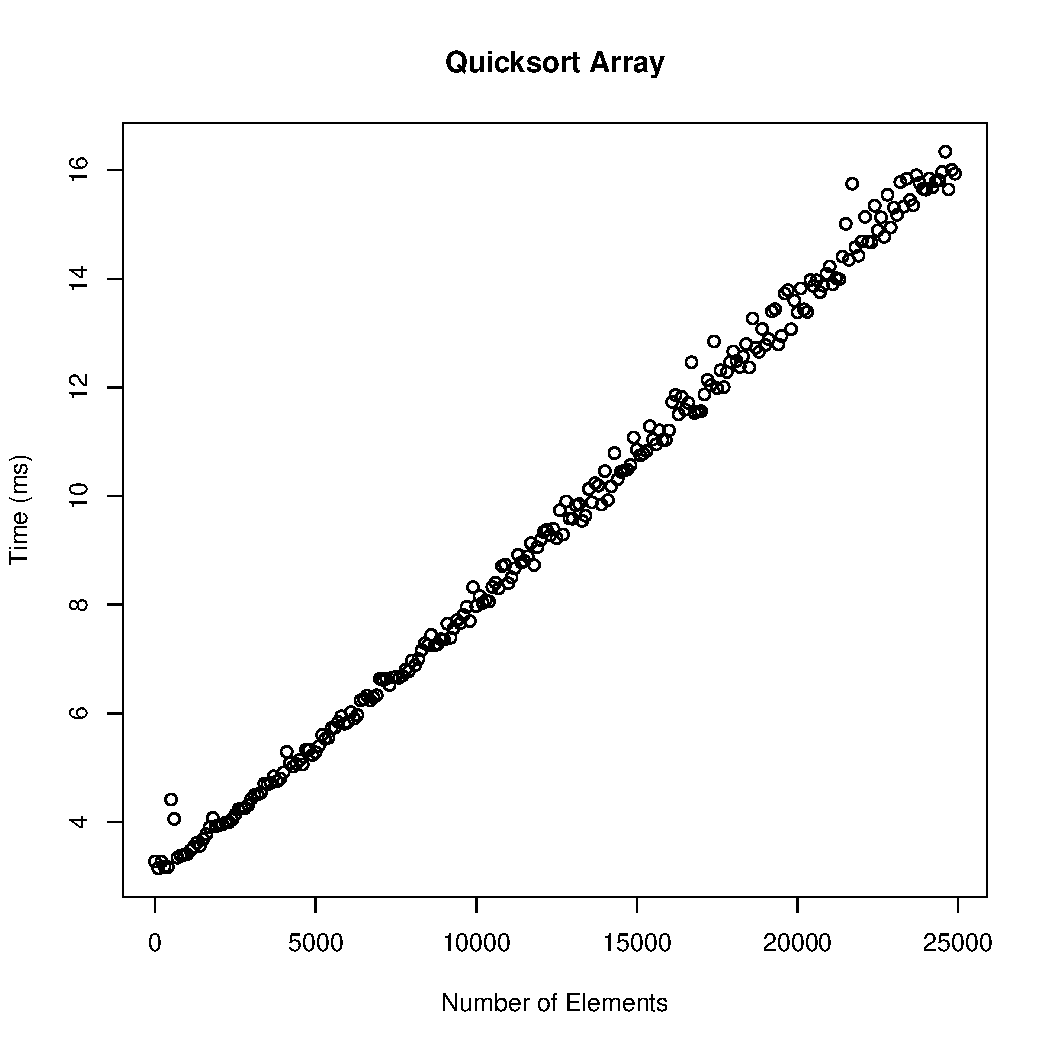
\includegraphics[height=10cm]{quicksort_array}
\subsection{Quicksort (Linked List)}
\subsubsection{Pseudocode}
\begin{verbatim}
proc quicksort(L, head, tail)
  if head ~= nil and tail ~= nil and head ~= tail
    pivot <- tail.val
    mid <- curr <- head
    last <- nil
    while curr ~= tail
      if curr.val < pivot
        swap curr.val and mid.val
        last <- mid
        mid <- mid.next
      curr <- curr.next
    if end.val < mid.val
      swap end.val and mid.val
    quicksort(A, start, last)
    quicksort(A, mid.next, end)
\end{verbatim}
\subsubsection{Benchmark Data}
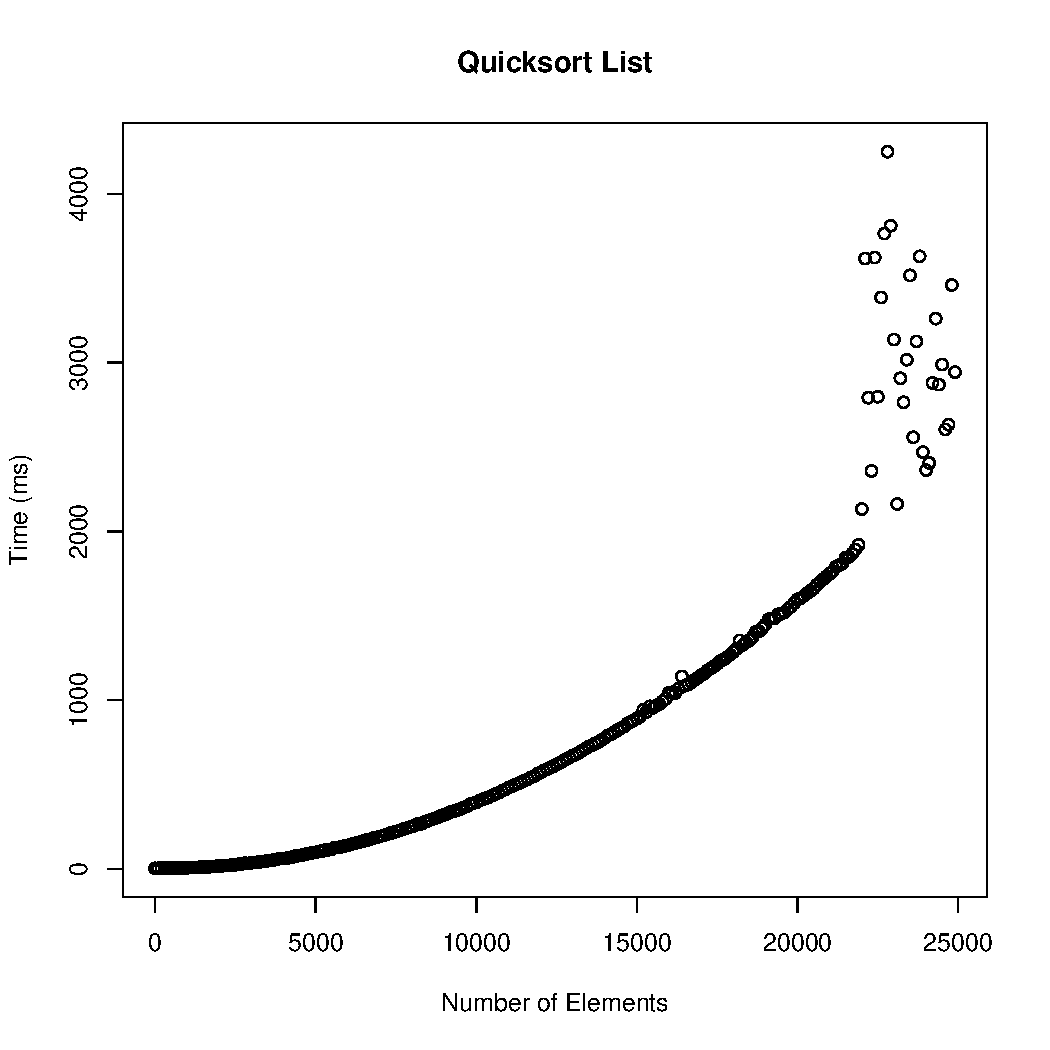
\includegraphics[height=10cm]{quicksort_list}
\subsection{Mergesort (Array)}
\subsubsection{Pseudocode}
\begin{verbatim}
proc mergesort(A)
  if A.length > 1
    divide A into A1 and A2
    mergesort(A1)
    mergesort(A2)
    merge(A1, A2, A)
proc merge(A1, A2, A)
  i <- 0
  j <- 0
  while i < A1.length or j < A2.length
    if i = A1.length
      A[i + j] <- A2[j]
      j++
    else if j = A2.length
      A[i + j] <- A1[i]
      i++
    else if A1[i] > A2[j]
      A[i + j] <- A1[i]
      i++
    else 
      A[i + j] <- A2[j]
      j++     
\end{verbatim}
\subsubsection{Benchmark Data}
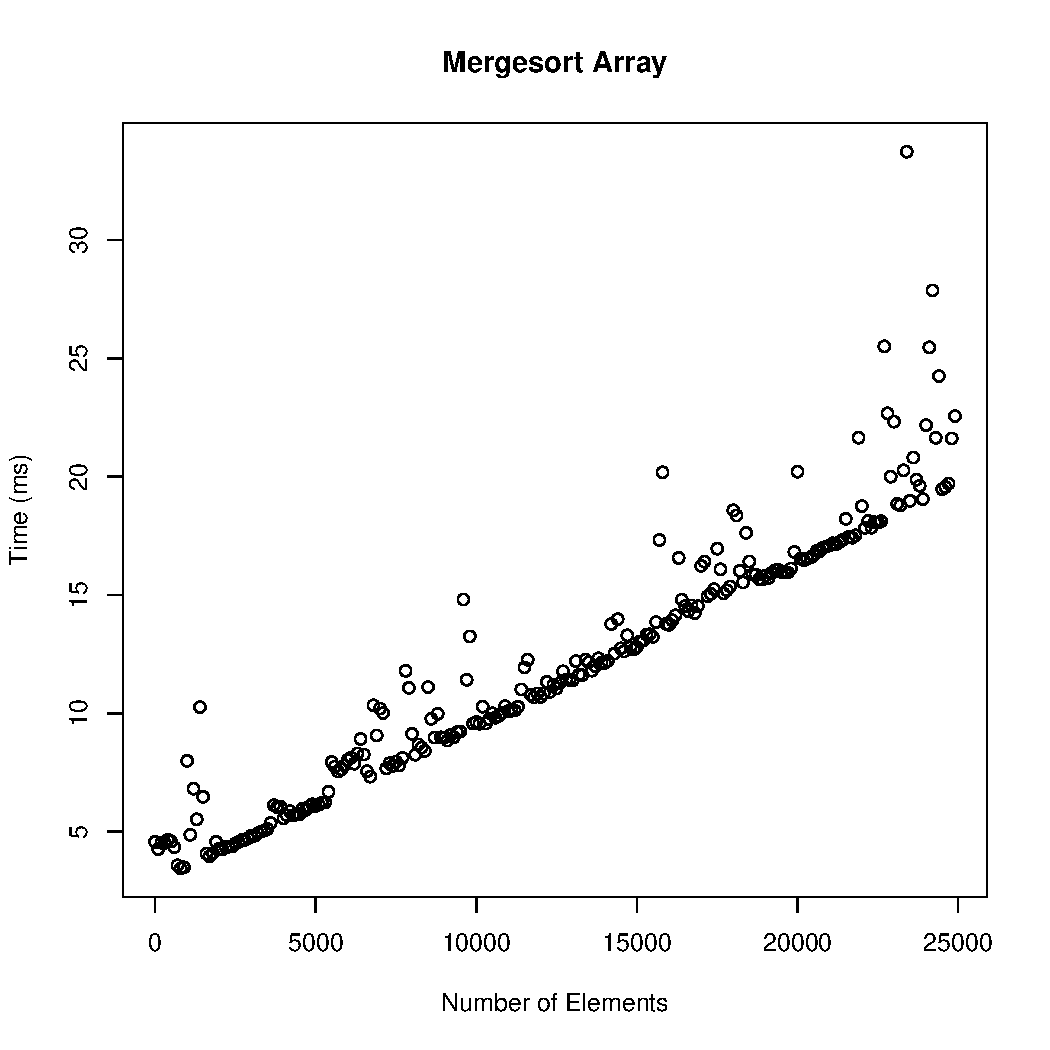
\includegraphics[height=10cm]{mergesort_array}
\subsection{Heapsort (Linked List)}
\subsubsection{Pseudocode}
\begin{verbatim}
proc mergesort(L)
  if L.next = nil
    split L into L1 and L2
    mergesort(L1)
    mergesort(L2)
    merge(L1, L2, L)
proc merge(L1, L2, L)
  curr <- L.head
  while L1 ~= nil and L2 ~= nil
    if L1 = nil
      curr.next <- L2
      L2 <- L2.next
    else if L2 = nil
      curr.next <- L1
      L1 <- L1.next
    else if L1.val > L2.val
      curr.next <- L2
      L2 <- L2.next
    else
      curr.next <- L1
      L1 <- L1.next
\end{verbatim}
\subsubsection{Benchmark Data}
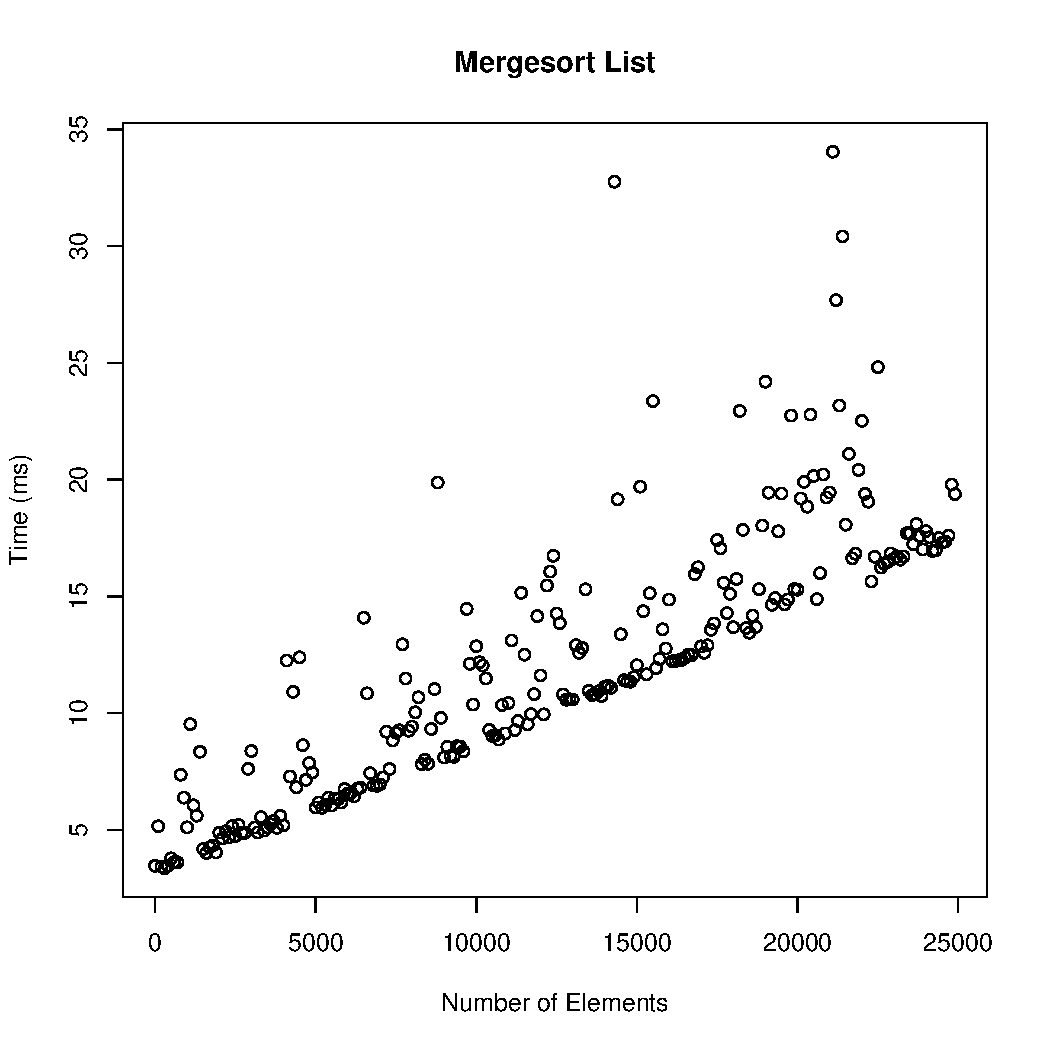
\includegraphics[height=10cm]{mergesort_list}
\section{Conclusion}
\end{document}
